	The client-side architecture follows the novel \gls{spa} paradigm. This approach proposes the creation of components to address a specific functionality of an interface. These components, based on a \gls{mvc} design pattern or any of its variations, are loaded dynamically when the user interacts with the Web application. Figure \ref{fig:design:ClientArchitecture}, represents the different parts that form a component (e.g. model, view and controller). The \gls{dom}, which is an object representation of the \gls{html} produced, is the place where the user sends any event such as clicking forward or backward buttons through an interview. These events are captured by controllers that perform tasks like keeping synchronised models and views. The models, used to represent the state of a component are best allocated to a single area since multiple views may initiate changes to them. Finally, the views reflect model data changes and contain the \gls{html} code that is rendered on the browser. In order to abstract the \gls{dom} manipulation every time a view changes, we use the popular AngularJS \footnote{\url{https://angularjs.org}} framework since it automatically handles the \gls{dom} control \cite{book:kozlowski13} and reduces the burden of testing components due to the different \gls{dom} implementations that browsers still have (e.g. Mozilla versus Internet Explorer).

	\begin{figure}[H]
	\centering
	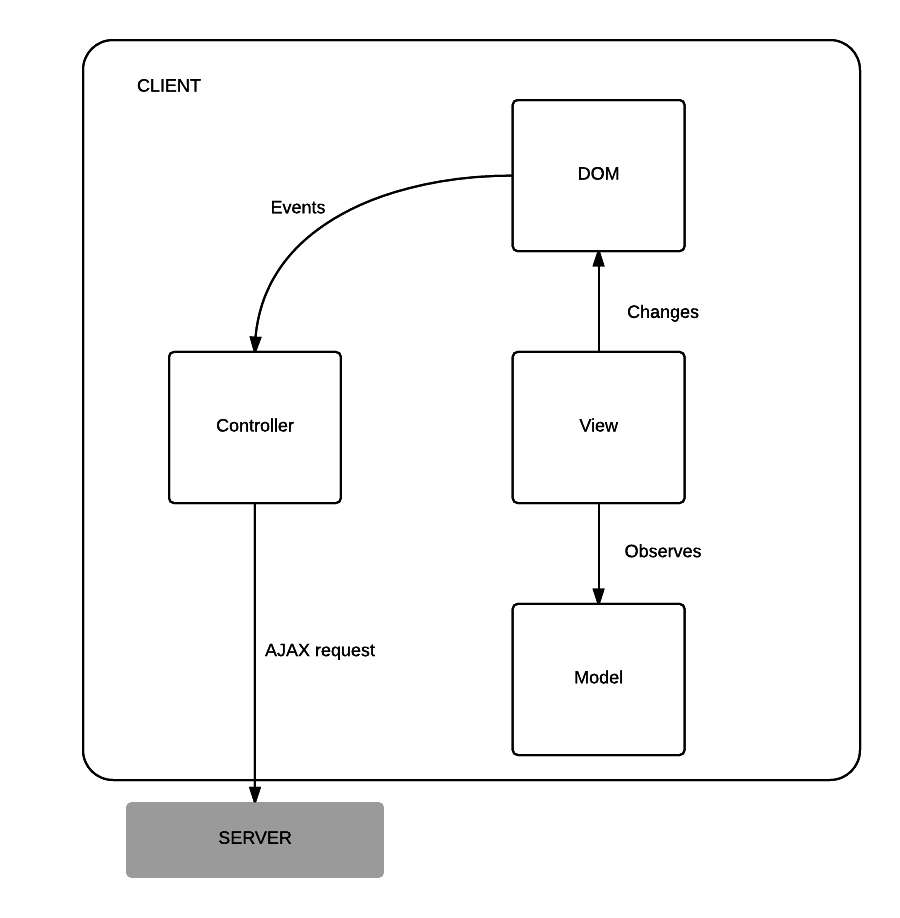
\includegraphics[width=0.75\textwidth]{design/img/webClientArchitecture.png}
	\caption{Client architecture}
	\label{fig:design:ClientArchitecture}
	\end{figure}

	Through the use of \gls{spa} paradigm, our server burden has been simplified since the task of building pages has been transferred to the client which has permitted obtaining rich interactive interfaces that do not need to be reloaded at every request. Moreover, the system has gained better responsiveness because the data transferred rather than being \gls{html} is \gls{json}, known for its compact syntax. Therefore, this solution stands out when compared to the multi-page paradigm that Blaise or SurveyMonkey have in which the entire interface is refreshed on every request \cite{proc:mesbah07} impacting not only over the system performance but also offering poorer user interactivity.


	

	



	